\chapter{System Design and Scheduling Algorithms}
\label{chap:system}

\section{System Architecture Overview}
\label{sec:system-architecture-overview}

The CGRSP evaluation system comprises five tightly coupled components (Figure~\ref{fig:architecture}). The components communicate through a single shared event queue: the Job Generator places arrival events, the DES Core dispatches them and invokes the Scheduler, the Scheduler queries the Fleet Manager for idle nodes, and the Metrics Collector receives completion notifications.



\begin{enumerate}
  \item \textbf{Job Generator}: produces a Poisson job stream with configurable arrival rate, complexity distribution, and deadline distribution.
  \item \textbf{Discrete-Event Simulator Core}: maintains a min-heap priority event queue and advances simulation time from event to event.
  \item \textbf{Fleet Manager}: tracks active instance slots up to $C_{\max}$, models per-type stock availability, and reports available slots to the scheduler. An ``idle'' slot has no GPU instance provisioned and incurs no cost; it represents unused concurrency capacity.
  \item \textbf{Scheduler}: implements the scheduling policy; receives the current queue and fleet state at each scheduling decision point and returns a list of (job, node) assignments.
  \item \textbf{Metrics Collector}: receives completion notifications and records per-job outcomes (waiting time, deadline adherence, cost) for reporting.
\end{enumerate}

The simulator core is adapted from SPARS~\cite{amrizal2026spars}, a lightweight discrete-event simulator for HPC job scheduling; its node power-state manager and energy accounting are replaced by the CGRSP fleet, stock-status provisioning model and QoS/cost metrics described in this chapter. The adapted simulator is implemented in Python using only the standard library and NumPy, so the build has no external simulation-framework dependency, which keeps full control over event semantics and metric computation.


\begin{landscape}
\begin{figure}[H]
\centering
\captionsetup{font=small,skip=6pt}
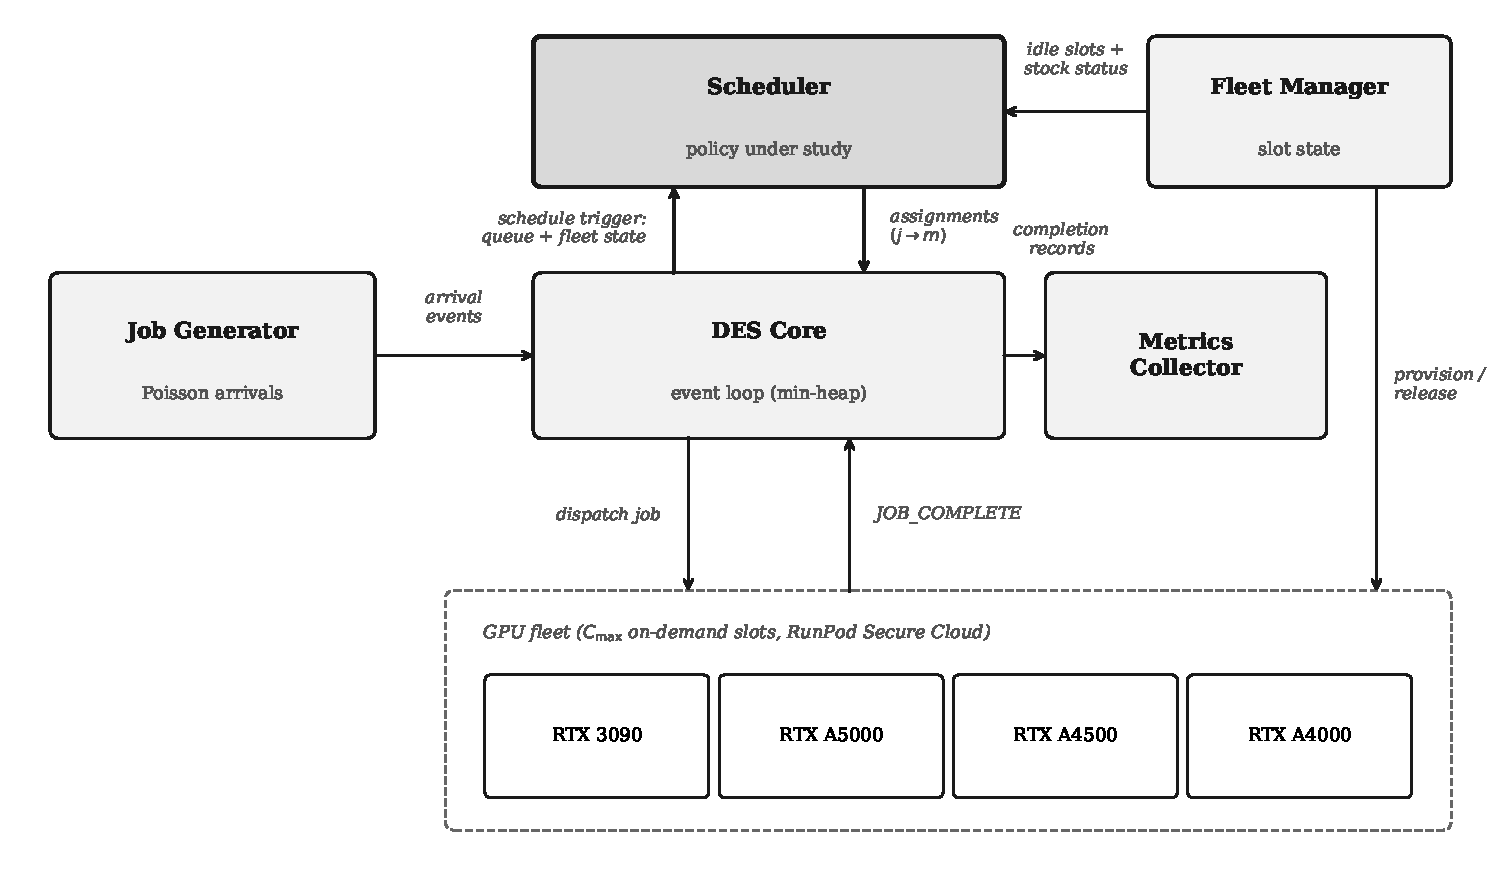
\includegraphics[width=0.98\linewidth,height=0.82\textheight,keepaspectratio]{figures/system_architecture.pdf}
\caption[CGRSP system architecture]{CGRSP system architecture: five components interact through a shared discrete-event queue. The Job Generator produces a Poisson job stream; the DES Core advances simulation time and invokes the Scheduler at each event; the Scheduler queries the Fleet Manager for idle slots and returns assignments; the Metrics Collector records per-job outcomes. The GPU fleet (dashed box) comprises four heterogeneous GPU types operating under stochastic stock-status provisioning-delay dynamics.}
\label{fig:architecture}
\end{figure}
\end{landscape}

\section{Discrete-Event Simulator Core}
\label{sec:discrete-event-simulator-core}

The simulator maintains a min-heap event queue ordered by event timestamp. Three event types drive the scheduling dynamics (the implementation also defines node transition, inert under the on-demand fleet, and simulation end, which closes every run; same-instant events are ordered by a priority field after the timestamp). The names below are descriptive aliases for the implementation's \texttt{JOB\_ARRIVAL}, \texttt{JOB\_COMPLETION} and \texttt{SCHEDULER\_DECISION}:

\begin{itemize}
  \item \texttt{JOB\_ARRIVAL}$(j, t)$: Job $j$ arrives at time $t$. The job is added to the waiting queue, and scheduling decision events are generated immediately (two at the same instant in the implementation, the second redundant for deterministic policies).
  \item \texttt{JOB\_COMPLETE}$(j, m, t)$: Job $j$ completes on node $m$ at time $t$. Node $m$ is freed, metrics are recorded, and a \texttt{SCHEDULE\_TRIGGER} event is generated.
  \item \texttt{SCHEDULE\_TRIGGER}$(t)$: The scheduler is invoked at time $t$. If any idle nodes and waiting jobs exist, the scheduler returns an assignment; the simulation then generates the corresponding \texttt{JOB\_COMPLETE} event at $t + \tau^{\text{prov}}_j + W(\kappa_j, g(m))$ (Eq.~\ref{eq:starttime}).
\end{itemize}

A job dispatched to a slot of type $g$ does not start instantly: it incurs a provisioning delay drawn from the stock-status-dependent range of Eq.~\ref{eq:provdelay} before entering the \textbf{running} state. No node-failure or node-restoration events occur, because the on-demand Secure Cloud pool never reclaims a held slot (Section~\ref{sec:problem-description}).

\section{GPU Fleet Model}
\label{sec:gpu-fleet-model}

The fleet manager instantiates nodes according to the GPU type configuration. Each node is parameterised by:

\begin{itemize}
  \item \textbf{GPU type} $g \in \calG$: determines $p_g$ and the execution time $W(\kappa, g)$.
  \item \textbf{Stock status}: High / Medium / Low, updated stochastically; it sets the provisioning delay (Eq.~\ref{eq:provdelay}; the status a scheduler observes is an independent, possibly stale draw from the same model, Section~\ref{ssec:platform-and-data}) and additionally informs node selection as a proxy for availability reliability, in scheduler-specific ways: EDF applies the stock tier as the \emph{primary} node-selection key (before execution time); CADR applies it as a \emph{hard filter}, excluding Low-stock types whenever an alternative exists; LCF weights it multiplicatively in its effective cost; and the SPT family, Balanced, and Adaptive add a stock penalty to their placement scores, whose Low-stock term is large enough to dominate the speed and cost terms; RH adds the same additive penalty to its placement score, where it acts as a tiebreaker among idle slots rather than a dominant term (see the node-selection paragraph of the RH description below).
  \item \textbf{Current state}: idle or running.
\end{itemize}

Table~\ref{tab:gpu_specs} shows the GPU fleet configuration used in all experiments. Pricing is the on-demand Secure Cloud price (\texttt{securePrice}) returned by the RunPod pricing API on 11~March 2026 (Taiwan time), the first snapshot of the author's 11~March to 20~April 2026 pricing-API collection (Figure~\ref{fig:availability-history}); RunPod does not publish a static per-GPU rate table in its documentation, and billing is per second~\cite{runpod2026podspricing}. The production pipeline that generated the empirical dataset ran instead on a RunPod Serverless endpoint. RunPod's default per-account Serverless worker quota is five workers~\cite{runpod2026maxworkers}, the value the experiments adopt as the baseline concurrency budget $C_{\max}=5$; the calibration data exclude every logged job that ran while more than five jobs were in flight (393 jobs), so the calibration record never exceeds the five-slot budget; the concurrency sweep of Section~\ref{ssec:concurrency-limit-sensitivity} treats larger budgets as simulated what-ifs. The job logs record no cost: the post-processing that assembled the August 2025 subset of the dataset (1,230 records, of which 1,031 remain after the concurrency exclusion) costed each job at RunPod's published Serverless Flex rates, \$0.684/hr for RunPod's 24\,GB tier (RTX~A5000, RTX~3090) and \$0.576/hr for its 16\,GB tier (RTX~A4000, and the 20\,GB RTX~A4500, which RunPod bills in that tier), while the 6,234-job calibration dataset lists the Pods \texttt{securePrice} for every job. The simulator deliberately prices each slot at that Pods \texttt{securePrice}, so its rates are lower than the Serverless Flex rates (by a factor of about 1.5 for the RTX~3090 and 2.3 to 2.5 for the A-series types), and a Serverless deployment would also pay for each job's scene-import phase, which the simulated service time excludes (Section~\ref{ssec:platform-and-data}). The Pods price ordering, with the RTX~3090 the most expensive type, is also not the Serverless one, under which the RTX~3090 and RTX~A5000 cost the same. The price is treated as a \textbf{fixed deterministic constant} throughout all simulations. RunPod prices are dynamic in practice and may differ at other points in time; the cost comparisons in this thesis are therefore valid as a snapshot analysis at that date, not as a prediction of future relative costs. The execution times derive from the 6,234-job empirical dataset.

\begin{table}[htbp]
\centering
\caption[GPU fleet configuration]{GPU types of the simulated fleet, priced at RunPod on-demand Secure Cloud rates. Prices are fixed deterministic values from the 11~March 2026 snapshot (RTX~A4500 and RTX~A4000 share the \$0.25/hr secure price at that date). Execution times from the 6,234-job empirical dataset; all experiments use $C_{\max}=5$ (RunPod's default per-account worker quota~\cite{runpod2026maxworkers}) as the baseline concurrency limit.}
\label{tab:gpu_specs}
\small
\begin{tabular}{lrrrrrr}
\toprule
\textbf{GPU Type} & \textbf{CUDA Cores} & \textbf{VRAM} & \textbf{Price (\$/hr)} & \textbf{Speed Rank}$^\dagger$ & \multicolumn{2}{c}{\textbf{Exec.\ Time (avg)}} \\
& & & & & Low $\kappa$ & High $\kappa$ \\
\midrule
RTX A5000 &  8,192 & 24\,GB & 0.27 & 1 & 60.7\,s & 94.5\,s \\
RTX 3090  & 10,496 & 24\,GB & 0.46 & 2 & 59.5\,s & 91.2\,s \\
RTX A4500 &  7,168 & 20\,GB & 0.25 & 3 & 62.0\,s & 88.3\,s \\
RTX A4000 &  6,144 & 16\,GB & 0.25 & 4 & 63.3\,s & 98.6\,s \\
\bottomrule
\end{tabular}
\vspace{6pt}
\raggedright\small $^\dagger$Speed rank by empirical average rendering time across all complexity levels (72.6, 72.9, 86.0, 98.4\,s for A5000, 3090, A4500, A4000 respectively; the A5000 and the 3090 differ by only 0.3\,s, so these averages do not separate their order). These averages are weighted by how each type's own jobs happen to be spread across the three complexity levels, not balanced across them, and the A4000's 249 jobs sit almost entirely at high complexity (247 of them), so its pooled average is close to a high-complexity average while the A5000's is not. The Speed Rank column should therefore be read as a summary of this particular workload mix rather than as a like-for-like speed ordering: at matched high complexity the ordering is the A4500 fastest, then the RTX~3090, the A5000, and the A4000 last. The simulator never uses these pooled averages; it draws service times from the per-stratum means $\overline{W}(\kappa, g)$ instead. The ranking is also non-monotone in CUDA cores: the RTX~A4500, despite having fewer cores than the 3090 and the A5000, has the lowest high-complexity ($\kappa=3$) stratum mean (88.3\,s, against 91.2\,s for the RTX~3090 and 94.5\,s for the A5000). These are observational stratum means, not scene-matched comparisons: GPU types were not randomised across scenes or dates, the A4000 jobs span only August to December 2025, and the A4500 shares no scene with another type. After the concurrency exclusion only two scenes are rendered on both the A4000 and the A5000 (a geometric-mean ratio of 1.165, indicative only), so no reliable scene-matched speed ratio exists, and the $\kappa=3$ ordering reflects this workload mix and should not be read as a hardware ranking. Low-$\kappa$ A4000/A4500 values are estimates (no low-complexity jobs for those types in the dataset).
\normalsize
\end{table}

The concurrency budget is realised as $C_{\max}$ on-demand rental slots (five on the experimental platform, Section~\ref{ssec:platform-and-data}). Each slot is a separate cloud instance that is rented, used for one job, and then released; when the job finishes the slot becomes free and is offered to the scheduler again. The fleet composition (the model parameter $n_g$) is fixed for the whole simulation. At construction the simulator assigns a GPU type to each of the $C_{\max}$ slots by round robin over the supported-type list (RTX~3090, RTX~A5000, RTX~A4500, RTX~A4000), which at $C_{\max}=5$ gives two RTX~3090 slots and one each of RTX~A5000, RTX~A4500, and RTX~A4000. A slot keeps its type for the entire run: the scheduler chooses \emph{which} slot to dispatch to, and thereby which GPU type a job runs on, but it never re-types a slot. This composition holds in every experiment except the concurrency-limit sensitivity study (Section~\ref{ssec:concurrency-limit-sensitivity}), which varies $C_{\max}$ and so re-runs the round-robin assignment for each $C_{\max}$ value.

The fixed composition is a modelling limitation worth stating explicitly, because it bounds what any scheduling policy can achieve. Exactly one slot carries the RTX~A5000, so at most one job at a time can occupy the type ranked fastest on the pooled averages of Table~\ref{tab:gpu_specs}, however strongly a speed-seeking policy prefers it; and two of the five slots carry the most expensive RTX~3090, so under saturation, when every slot is busy, two fifths of the concurrent work runs on the costliest type whatever the policy decides. A fleet whose idle slots could be re-provisioned to a different type on demand would give the cost-aware and speed-aware policies a larger decision space than they have here. The comparisons reported in Chapter~\ref{chap:experiments} are therefore conditional on this fixed heterogeneous mix, and are not claims about a fleet free to re-provision.

Execution times are modelled stochastically. When a job of complexity level $\kappa \in \{1, 2, 3\}$ is dispatched to GPU type $g$, its realised render time is drawn from a log-normal distribution $W(j,g) \sim \text{LogNormal}(\mu_{\kappa,g}, \sigma_{\kappa,g}^2)$ whose expected value equals the mean execution time $\overline{W}(\kappa, g)$ of the corresponding $(\kappa, g)$ stratum in the empirical dataset (Eq.~\ref{eq:servicetime}; the fitted parameters are given in Section~\ref{ssec:platform-and-data}, Eq.~\ref{eq:lognormal}). The within-stratum dispersion $\sigma_{\kappa,g}$ is fitted directly from the data as the standard deviation of $\ln(\text{render time})$ within each stratum (pooled $\sigma_{\ln} \approx 0.11$; strata with fewer than five observations use the pooled value). The log-normal form respects the strictly positive, right-skewed shape of the empirical measurements, with a minority of jobs running substantially longer than the mean (outliers from complex geometry or large textures). Schedulers plan with the expected service time $\overline{W}(\kappa_j, g)$ as the estimate $e_j$, since the exact walltime of a job is not observable at dispatch; only the realised completion time is stochastic. The realised execution time is sampled from a per-simulation random stream seeded independently of the provisioning-delay draws, so that scheduler comparisons remain reproducible and differences are attributable to scheduling policy.

\section{Job Generator}
\label{sec:job-generator}

Jobs arrive according to a Poisson process with configurable mean rate $\lambda$ (jobs/second); each job is one frame (Chapter~\ref{chap:formulation}). The Poisson assumption is standard for independent job-submission workloads: jobs originate from different clients and scenes, making submissions memoryless with exponentially distributed inter-arrival times, the canonical model for computer system workloads~\cite{banks2010discrete}. Each job is independently assigned:

\begin{itemize}
  \item \textbf{Complexity} $\kappa_j \in \{1, 2, 3\}$: sampled from the calibration distribution (32.92\% low, 34.12\% medium, 32.96\% high), based on the per-stratum counts (2,052 / 2,127 / 2,055 of 6,234) obtained by classifying the filtered CSV at the rounded 65.2\,s and 73.9\,s thresholds with strict less-than. The split is close to thirds because the thresholds approximate the 33rd and 67th percentiles of render time. Because $\kappa$ is therefore an ex-post label derived from the measured render time (the dataset holds no ex-ante predictor of it; total pixels correlate with render time at only $-0.04$), the simulator treats it as known at arrival, so every policy plans with a tercile that already reflects the job's realised duration class. The within-stratum dispersion of the densely observed low and medium strata is small, but the log-normal draws are not truncated at the tercile boundaries and the sparse cells use the pooled $\sigma_{\ln}$, so roughly one simulated draw in five lands outside its label's tercile. Results therefore describe a dispatcher that can classify a scene's complexity before rendering, and are an optimistic case for the policies that use the class (the point-estimate miss rates of RH, CADR, SPT and SPT+Rescue are higher in the degraded-label arms than at baseline, though not monotonically and for most arms not significantly on a paired test, whereas EDF's is lower in every label arm); Section~\ref{ssec:label-noise-and-gpu-speed-assumptions} brackets the degradation.
  \item \textbf{Deadline} $d_j = t_j^{\text{submit}} + T_j$, $T_j \in \{T_{\text{tight}}, T_{\text{loose}}\}$ (Eq.~\ref{eq:deadline_window}): in the baseline scenario each job draws either the tight deadline window $T_{\text{tight}}$ (rush-order renders) or the loose window $T_{\text{loose}}$ (standard batch renders); the values and class proportions are the platform parameters of Section~\ref{ssec:platform-and-data}. The tight/loose split is held constant across all day types; load intensity is varied through $\lambda$ and the total job count $N_{\text{jobs}}$ (Section~\ref{ssec:platform-and-data}) only.
  \item \textbf{Estimated duration}: a fixed 100\,s placeholder recorded as job metadata and read by no scheduler; schedulers compute their own per-node estimates $\overline{W}(\kappa_j, g(m))$ at dispatch (Section~\ref{ssec:spt-shortest-processing-time}).
\end{itemize}

\section{Scheduling Algorithms}
\label{sec:scheduling-algorithms}

All ten scheduling algorithms implement the same interface: they receive the current waiting job queue and fleet state, and return a list of (job, node) assignments (zero or more, executed simultaneously for multiple idle nodes).

\subsection{FIFO: First-In-First-Out}
\label{ssec:fifo-first-in-first-out}

FIFO assigns waiting jobs to idle nodes in submission-time order (earliest submit time first), as summarised in Algorithm~\ref{alg:fifo}. Node selection among idle nodes is arbitrary (earliest-registered first in the implementation). FIFO serves as the primary baseline because it requires no job characteristic knowledge and is deadline-oblivious.

\begin{algorithm}[H]
\caption{FIFO Scheduler}
\label{alg:fifo}
\begin{algorithmic}[1]
\REQUIRE Queue $Q$ sorted by $t_j^{\text{submit}}$; set $I$ of idle nodes
\STATE Sort $Q$ by $t_j^{\text{submit}}$ ascending
\FOR{each $(j, m)$ in $\text{zip}(Q, I)$}
  \STATE Assign job $j$ to node $m$
\ENDFOR
\end{algorithmic}
\end{algorithm}




\subsection{SPT: Shortest Processing Time}
\label{ssec:spt-shortest-processing-time}

SPT prioritises the job with the smallest expected execution time, computed at each event as $e_j = \min_{m \in I} \overline{W}(\kappa_j, g(m))$ over the currently idle capable nodes, so the ranking always reflects the fleet actually available at dispatch. Jobs with equal $e_j$ (the common case, since $e_j$ takes one of three values per node type) keep the queue's earliest-deadline, then earliest-arrival order, so SPT is deadline-blind across complexity classes but not within one; the same tie rule applies to every SPT-ordered tier in the SPT+Rescue, CADR and Adaptive policies. (The job metadata also carries a fixed 100\,s placeholder duration, which no scheduler reads.) Because all three complexity levels are calibrated to the same reference GPU, SPT naturally front-loads the shortest (low-complexity) jobs, reducing the mean number of jobs in the queue at any instant, the discrete-time analogue of the M/G/1 SPT optimality result~\cite{pinedo2016scheduling}.

Node selection: given the sorted job queue, SPT assigns each job to the idle node minimising a normalised composite of speed, cost, and stock reliability of the same structural form as the Balanced score (Eq.~\ref{eq:balanced_score}),
\begin{equation}
\text{score}(j,m) = (1 - w_c)\,\frac{\overline{W}(\kappa_j, g(m))}{\overline{W}_{\min}(j)} + w_c\,\frac{p_{g(m)}}{p_{\min}} + \text{sp}(s_m),
\label{eq:spt_score}
\end{equation}
with cost weight $w_c = 0.3$, where $\overline{W}_{\min}(j)$ is the fastest expected execution time for job $j$ across the idle nodes, $p_{\min}$ the cheapest per-second rate among them, and $\text{sp}(s_m) \in \{0, 0.2, 1.0\}$ a High/Medium/Low stock-status penalty (writing $s_m$ as shorthand for the stock status $s_{g(m)}(t)$ of the node's type). Speed carries the larger weight ($0.7$), so the fastest node is selected unless a marginally slower node is sufficiently cheaper or more reliably stocked to overcome the speed term; when cost and stock are uniform across the idle nodes the rule reduces to the minimum-completion-time (fastest-finish) heuristic of~\cite{braun2001comparison} applied within each scheduling decision. Algorithm~\ref{alg:spt} summarises the procedure.

\begin{algorithm}[H]
\caption{SPT Scheduler}
\label{alg:spt}
\begin{algorithmic}[1]
\REQUIRE Queue $Q$; idle node set $I$; current time $t$
\STATE Sort $Q$ ascending by $e_j = \min_{m \in I} \overline{W}(\kappa_j, g(m))$
\FOR{each job $j$ in $Q$}
  \IF{$I = \emptyset$} \STATE \textbf{break} \ENDIF
  \STATE $m^* \leftarrow \arg\min_{m \in I}\; \big[(1{-}w_c)\tfrac{\overline{W}(\kappa_j, g(m))}{\overline{W}_{\min}(j)} + w_c\tfrac{p_{g(m)}}{p_{\min}} + \text{sp}(s_m)\big]$ \COMMENT{Eq.~\ref{eq:spt_score}, $w_c{=}0.3$}
  \STATE Assign $j \to m^*$; remove $m^*$ from $I$
\ENDFOR
\end{algorithmic}
\end{algorithm}

\subsection{EDF: Earliest Deadline First}
\label{ssec:edf-earliest-deadline-first}

EDF prioritises the job with the nearest absolute deadline $d_j$. When two jobs have the same deadline, submission time is used as a tiebreaker. Node selection minimises the expected execution time $\overline{W}(\kappa_j, g(m))$ for the job's specific complexity level, with stock-availability tiers applied first (High $\prec$ Medium $\prec$ Low). Using job-specific execution times (rather than a generic speed multiplier) is necessary because GPU rank varies by complexity: for example, RTX~A4500 (88.3\,s) outperforms RTX~3090 (91.2\,s) on high-complexity jobs despite fewer CUDA cores.

\subsection{LCF: Lowest Cost First}
\label{ssec:lcf-lowest-cost-first}

LCF minimises total operational cost by preferring the cheapest available GPU type. Node selection uses an effective cost score $c_{\text{eff}}(j,m) = p_{g(m)} \cdot \overline{W}(\kappa_j, g(m)) \cdot \psi(s_m)$, where $\psi(s_m) \in \{1.0, 1.05, 1.15\}$ is a stock-status penalty (High/Medium/Low stock) reflecting availability reliability. Job ordering within LCF is by submission time (FIFO order).

The stock-status penalty ensures that when two GPUs have the same rental price, the one with higher availability reliability is preferred, avoiding types that are likely to be scarce and so incur a long provisioning delay.

\subsection{Balanced: Weighted Speed-Cost Composite}
\label{ssec:balanced-weighted-speed-cost-composite}

Balanced assigns a composite score to each (job, node) pair:

\begin{equation}
\text{score}(j, m) = w_b \cdot \frac{\overline{W}(\kappa_j, g(m))}{\overline{W}_{\max}(j)} + (1-w_b) \cdot \frac{p_{g(m)}}{p_{\max}} + \text{sp}(s_m)
\label{eq:balanced_score}
\end{equation}

where $w_b = 0.8$ (speed-biased), $\overline{W}_{\max}(j)$ is the maximum execution time for job $j$ across all fleet nodes (per-job normalisation), $p_{\max}$ is the global maximum per-second cost across the fleet, and $\text{sp}(s_m) \in \{0.0, 0.2, 1.0\}$ is a stock-status penalty. The job ordering within Balanced is by submission time (FIFO), so Balanced's differentiation from FIFO comes entirely from its node selection score. This is deliberately distinct from EDF's deadline-based job ordering.

\subsection{Random: Random Baseline}
\label{ssec:random-random-baseline}

Random selects both job and node uniformly at random from the available sets. It serves as a lower-bound baseline to verify that the structured heuristics provide a benefit over chance.

\subsection{Design Progression}
\label{ssec:design-progression}

The ten scheduling algorithms evaluated in this study represent a progressive refinement of deadline awareness and wait minimisation. FIFO provides the deadline-oblivious baseline. SPT reduces mean wait by front-loading short jobs but remains deadline-blind. SPT+Rescue introduces the laxity rescue concept: a secondary EDF tier that promotes jobs whose deadline slack has fallen below a threshold. The Adaptive scheduler (Section~\ref{ssec:adaptive-queue-pressure-edf-spt-hybrid}) extends that idea with a hopeless tier and a queue-pressure rule that widens the urgent tier under congestion, interpolating between SPT and EDF. The Rolling-Horizon scheduler (Section~\ref{ssec:anticipative-rolling-horizon-scheduler}) goes further: instead of a hand-set slack threshold it plans over the slot-availability timeline and anticipated arrivals, keeping fixed tier orders (SPT, EDF, demote-last) but promoting a job only when the timeline shows it would otherwise miss. The CADR scheduler (Section~\ref{ssec:cadr-cost-aware-deadline-risk}) introduces a scale-free critical-ratio triage that achieves near-RH miss performance while substantially reducing the tardiness (lateness) of missed deadlines by promoting at-risk jobs earlier, so that fewer tight jobs slip into the demoted tier. Figure~\ref{fig:scheduler-lineage} summarises this lineage: each arrow marks the algorithmic ingredient added at that step, and the two proposed schedulers (RH and CADR) both descend from SPT+Rescue.

\begin{landscape}
\begin{figure}[H]
\centering
\captionsetup{font=small,skip=6pt}
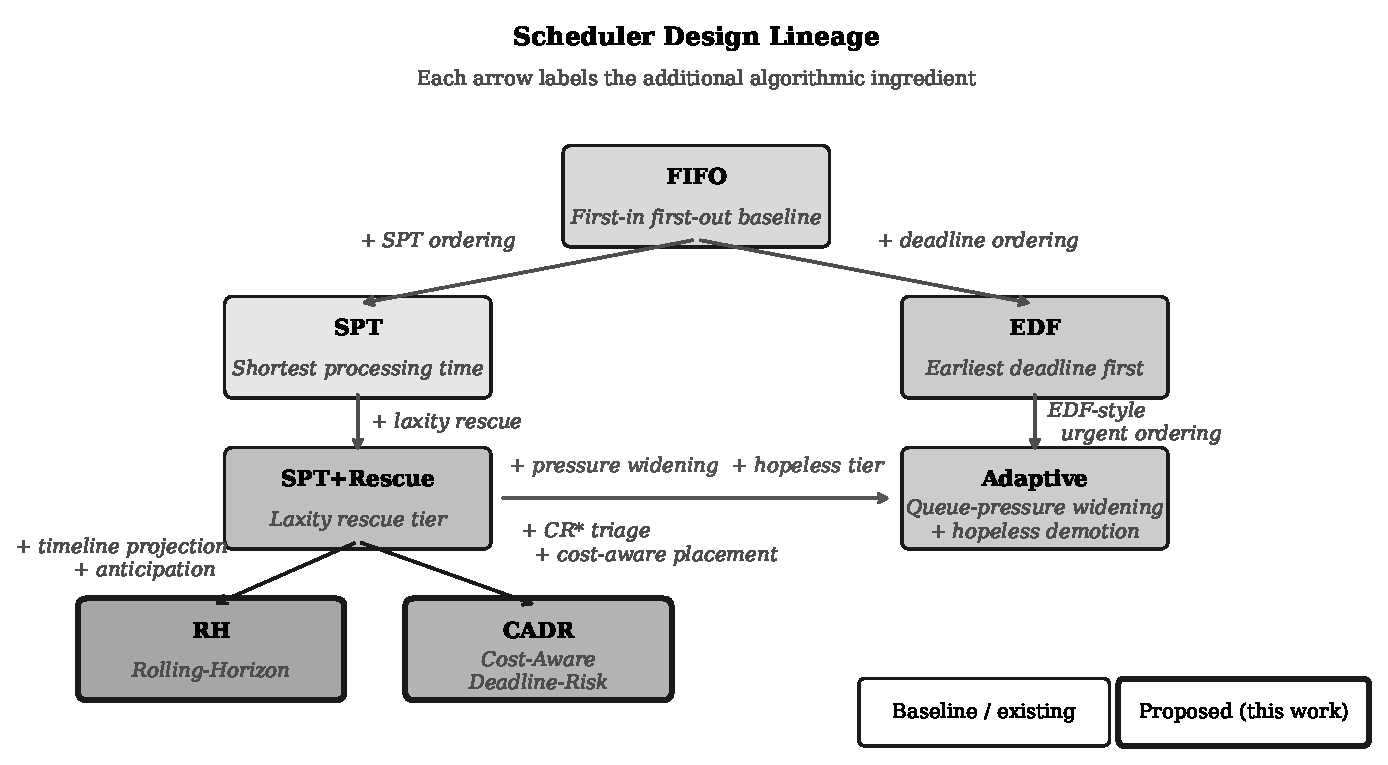
\includegraphics[width=0.98\linewidth,height=0.72\textheight,keepaspectratio]{figures/scheduler_lineage.pdf}
\caption[Scheduler design lineage]{Scheduler design lineage. Each arrow labels the algorithmic ingredient added at that step. FIFO is the deadline-oblivious baseline; SPT adds shortest-job-first ordering to reduce wait; EDF adds deadline ordering to reduce misses; SPT+Rescue adds a laxity rescue tier to combine both effects; the Adaptive hybrid extends the rescue tier with queue-pressure tier widening and hopeless demotion; the proposed RH scheduler replaces the hand-set slack threshold with a boundary read from a forward timeline projection and adds load-gated anticipation; the proposed CADR scheduler replaces the laxity threshold with a scale-free critical-ratio triage and adds cost-aware node selection.}
\label{fig:scheduler-lineage}
\end{figure}
\end{landscape}

\subsection{SPT+Rescue: Hybrid Throughput-Deadline Policy}
\label{ssec:spt-rescue-hybrid-throughput-deadline-policy}

SPT+Rescue introduces the laxity rescue concept as an intermediate design step. It combines SPT's wait-time advantage with an EDF-based deadline rescue mechanism: most jobs are ordered by shortest processing time, but any job whose \emph{laxity} drops below a threshold is promoted to an urgent tier and dispatched before all normal-tier jobs.

The laxity of job $j$ at scheduling decision time $t$ is defined as:
\begin{equation}
L_j(t) = d_j - t - \min_{m \in I}\, \overline{W}(\kappa_j, g(m))
\label{eq:laxity}
\end{equation}
where the minimum is taken over all currently idle nodes $I$. Laxity measures the slack remaining: if $L_j(t) < 0$, even immediate dispatch on the fastest idle node misses under the mean service-time estimate, but a shorter realised execution time can still meet the deadline; small positive laxity signals risk if dispatch is deferred.

At each scheduling event the scheduler partitions the waiting queue into two tiers (Figure~\ref{fig:rescue-flow}):
\begin{itemize}
  \item \textbf{Urgent} ($L_j < \theta$): sorted by earliest absolute deadline (EDF order within tier)
  \item \textbf{Normal} ($L_j \geq \theta$): sorted by shortest estimated processing time (SPT order)
\end{itemize}

\begin{landscape}
\begin{figure}[H]
\centering
\captionsetup{font=small,skip=6pt}
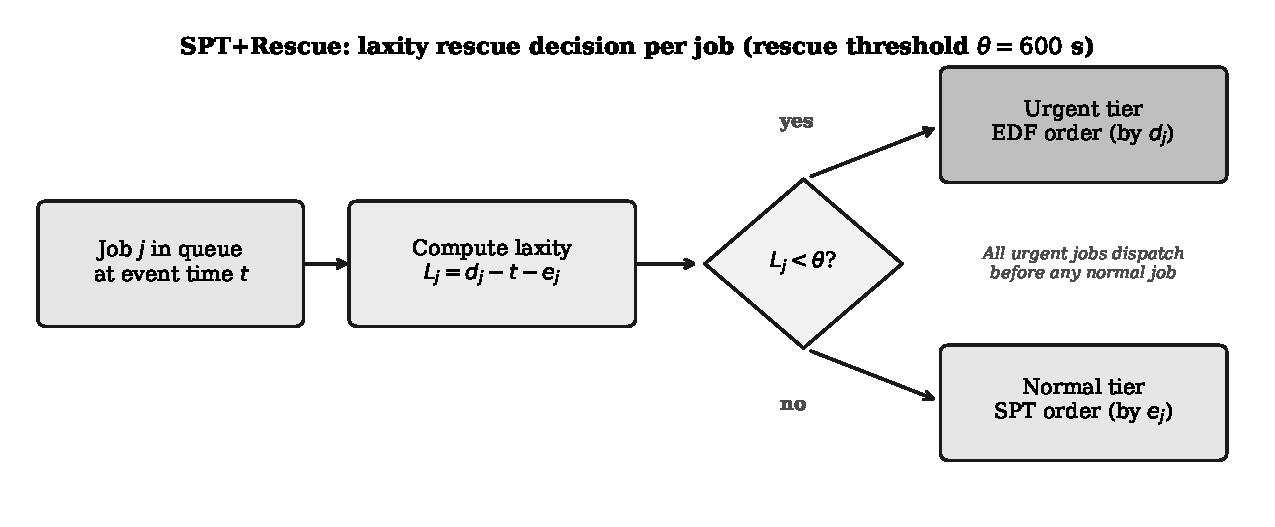
\includegraphics[width=0.98\linewidth,height=0.72\textheight,keepaspectratio]{figures/rescue_flow.pdf}
\caption[SPT+Rescue laxity rescue decision flow]{SPT+Rescue per-job decision flow. At each scheduling event, every queued job's laxity $L_j = d_j - t - e_j$ is computed against the fastest available execution time; jobs with laxity below the rescue threshold $\theta$ enter the urgent tier (EDF order), the rest stay in the normal tier (SPT order), and all urgent jobs dispatch before any normal job.}
\label{fig:rescue-flow}
\end{figure}
\end{landscape}
All urgent jobs are dispatched before any normal-tier job. The rescue threshold is set to $\theta = 600$\,s (10 minutes) in all experiments. This value was chosen by the following reasoning: by the laxity definition (Eq.~\ref{eq:laxity}), a job that has just crossed the rescue threshold has laxity exactly $\theta$, so dispatching it immediately leaves exactly $\theta = 600$\,s to spare before the deadline, comfortably above even a high-complexity job's empirical 99th-percentile render time (about 150\,s; the observed maximum is about 350\,s). The margin covers render-time variability and a High or Medium stock provisioning delay (at most 120\,s), but not a Low-stock delay (at least 600\,s), which the model can draw during peak hours. A sensitivity study over $\theta \in \{60, 180, 300, 600, 1200\}$\,s (Section~\ref{ssec:rescue-threshold-sensitivity}) ($n=10$ seeds) shows that miss rate varies by \ThrMissSpread\,percentage points across the whole swept range, a little over half of it from the shortest threshold: $\theta=60$\,s is the weakest, whereas the four values $\theta \ge 180$\,s lie within about two percentage points of each other, a spread comparable to the seed noise at this sample size. The sweep minimum lies at $\theta=180$\,s, so the default $\theta=600$\,s sits on the flat part of the curve and requires no tuning. Algorithm~\ref{alg:sptrescue} summarises the two-tier procedure.

\begin{algorithm}[H]
\caption{SPT+Rescue Scheduler}
\label{alg:sptrescue}
\begin{algorithmic}[1]
\REQUIRE Queue $Q$; idle node set $I$; current time $t$; threshold $\theta$
\FOR{each job $j \in Q$}
  \STATE $e_j \leftarrow \min_{m \in I} \overline{W}(\kappa_j, g(m))$ \COMMENT{fastest available expected exec time}
  \STATE $L_j \leftarrow d_j - t - e_j$
\ENDFOR
\STATE $Q_{\text{urgent}} \leftarrow \{j \in Q : L_j < \theta\}$, sorted by $d_j$ ascending
\STATE $Q_{\text{normal}} \leftarrow \{j \in Q : L_j \geq \theta\}$, sorted by $e_j$ ascending
\FOR{each job $j$ in $Q_{\text{urgent}} \mathbin{\|} Q_{\text{normal}}$}
  \IF{$I = \emptyset$} \STATE \textbf{break} \ENDIF
  \STATE $m^* \leftarrow \arg\min_{m \in I} \big[(1{-}w_c)\tfrac{\overline{W}(\kappa_j, g(m))}{\overline{W}_{\min}(j)} + w_c\tfrac{p_{g(m)}}{p_{\min}} + \text{sp}(s_m)\big]$ \COMMENT{Eq.~\ref{eq:spt_score}, $w_c{=}0.3$}
  \STATE Assign $j \to m^*$; remove $m^*$ from $I$
\ENDFOR
\end{algorithmic}
\end{algorithm}

SPT+Rescue combines SPT's shortest-job-first ordering with EDF deadline rescue: under capacity saturation it achieves \RescueMiss\% miss (notably lower than SPT's \SPTmiss\%) at \RescueWait~min wait ($d=\RescueFIFOwaitD$ vs FIFO, $p<0.001$), providing a conservative fallback when tight-deadline compliance is a strict operational requirement.

\subsection{Illustrative Scheduling Example}
\label{ssec:illustrative-scheduling-example}

Figure~\ref{fig:gantt} traces a concrete 7-job scenario with $C_{\max}=3$ nodes (a minimal illustrative configuration chosen so that all 7 jobs queue up and the rescue decision is visible; the baseline experiments use $C_{\max}=5$, and the concurrency sweep varies it) to show how SPT+Rescue differs from FIFO in a single scheduling window. Only J6 carries an illustrative tight deadline ($d_6=210$\,s, 160\,s after its arrival at $t=50$\,s; $\kappa_6=2$, medium complexity); this deliberately shortened window makes the rescue decision visible and is not the baseline one-hour tight window used in the experiments. All other jobs have loose (8-hour) deadlines. The illustrative scenario sets provisioning delay to zero and uses approximated, complexity-uniform execution times matching the figure legend ($\kappa{=}1\approx65$\,s, $\kappa{=}2\approx75$\,s, $\kappa{=}3\approx120$\,s, the last chosen for narrative clarity rather than as a close rounding of the empirical high-complexity mean). J0, J1, J2 arrive in the first 10\,s and fill all three nodes immediately; J3 to J6 queue while all nodes are busy. When node N1 becomes free at $t=70$\,s, FIFO dispatches J3 (next in arrival order), then at $t=75$\,s dispatches J4 to N2, eventually assigning J6 to N2 at $t=140$\,s. J6 finishes at 215\,s, 5\,s past its deadline ($\delta_6=0$). SPT+Rescue instead evaluates laxity when N1 frees at $t=70$\,s (the sole idle node at that moment; $\overline{W}(\kappa_6{=}2, g(\text{N1}))=75$\,s):
\begin{equation}
  L_{J_6}(70) = d_6 - 70 - \min_{m \in I} \overline{W}(\kappa_6, g(m)) = 210 - 70 - 75 = 65\,\text{s}
\end{equation}
Since $65$\,s is below the $600$\,s rescue threshold, J6 is classified urgent and dispatched immediately to N1. J6 starts at $t=70$\,s and finishes at 145\,s, meeting its deadline by 65\,s ($\delta_6=1$). Loose-deadline jobs J3 to J5 are reordered by SPT without any deadline impact.

\begin{landscape}
\begin{figure}[H]
\centering
\captionsetup{font=small,skip=6pt}
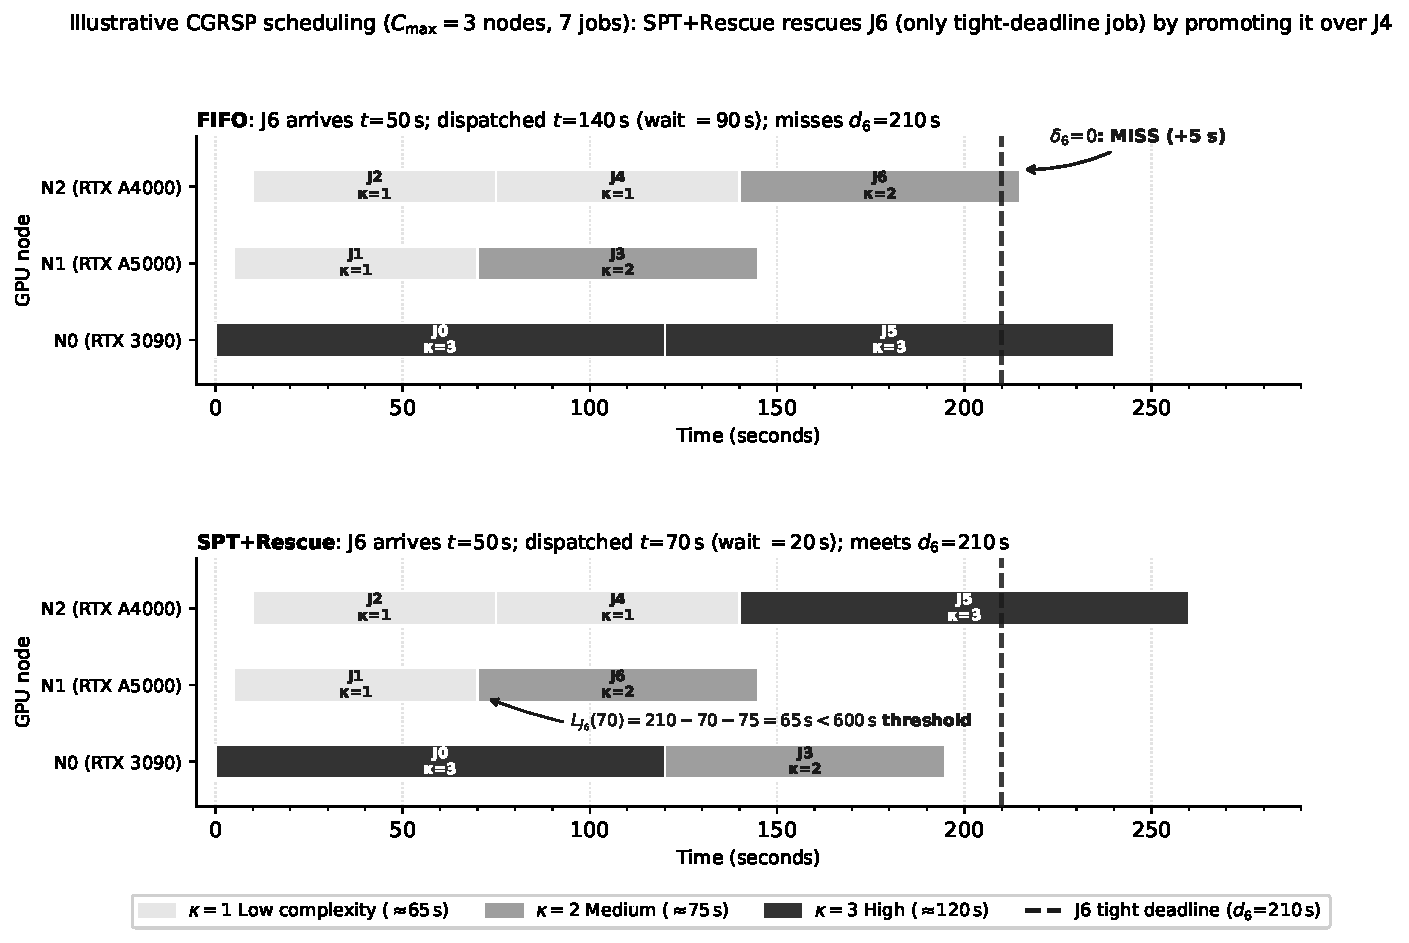
\includegraphics[width=0.98\linewidth,height=0.88\textheight,keepaspectratio]{figures/gantt_chart.pdf}
\caption[Illustrative Gantt chart: FIFO vs SPT+Rescue]{Illustrative Gantt chart: FIFO vs SPT+Rescue.}
\label{fig:gantt}
\end{figure}
\end{landscape}


\subsection{Anticipative Rolling-Horizon Scheduler}
\label{ssec:anticipative-rolling-horizon-scheduler}

The Rolling-Horizon (RH) scheduler is the first, and methodologically the more novel, of the two scheduling contributions of this work. Rather than ranking the queue by a single fixed priority rule, it projects the near-future availability of the fleet and dispatches against that projection. At each scheduling event it builds the availability timeline of every usable slot (idle now, or busy until its running job's expected completion), classifies each waiting job by whether the timeline shows it would still meet its deadline if it deferred to the next slot to free, and then greedily places jobs, in that urgency order, each onto the slot that minimises a per-job weighted-sum surrogate of the model objective (Eq.~\ref{eq:objective}), namely the projected value, under the planning estimate $e_j$ in place of the realised $W$, of $w_{\text{qos}}(\alpha_1 w_j + \alpha_2 (1-\delta_j)) + w_{\text{cost}}\,c_j$ with $w_{\text{qos}}=w_{\text{cost}}=0.5$ (the explicit form is given in Algorithm~\ref{alg:rh}). The score additionally includes a stock-status penalty and a fixed per-type reliability prior. Thus a tie in projected QoS does not guarantee that the lowest-cost node wins; this is a heuristic approximation of, not an exact solution to, the lexicographic objective. It commits only the dispatches that start at the current instant and re-plans at the next event, in the manner of receding-horizon (model-predictive) control. The placement step is a greedy, per-job assignment rather than a joint optimisation over the horizon; the tier orders themselves are fixed rules (shortest processing time first for normal jobs, earliest deadline first for urgent jobs, doomed jobs last), and what is novel is that the boundary between the urgent and normal tiers is read from the projected slot timeline, adapting to the realised fleet state, instead of from a hand-set laxity threshold. The scheduler is additionally anticipative: below saturation it reserves a little capacity for imminent tight-deadline arrivals (described below).

The RH scheduler is anticipative but not clairvoyant: it knows the job arrival-rate profile and the deadline-window distribution (operational statistics estimable from a studio's own submission history), but it does not observe the identities or submission times of jobs that have not yet arrived. This is the standard distinction in online stochastic optimisation between distributional knowledge and realisation knowledge: the scheduler may reserve capacity for the \emph{expected} rate of imminent tight-deadline arrivals, never for specific future jobs.

That the arrival rate is estimable in principle does not make the policy indifferent to how well it is estimated, and the sensitivity has an unusual shape that a practitioner needs to know about. The assumed $\lambda$ enters the policy at exactly one place, the load gate of the anticipation mechanism described below, and the gate is a step function: it compares $\rho = \lambda\,\overline{W}/C_{\max}$ against $\rho_{\text{gate}}$, which at $C_{\max}=5$ puts the switching point at $\lambda \approx \PriorGateLambda$~jobs/s, only about \PriorGateShortfall\% below the hectic day's true rate of $0.100$~jobs/s. A 30-seed sweep in which RH is given a deliberately mis-estimated arrival rate, swept as a multiple of the true $\lambda$ on the hectic and surge days, confirms both halves of this shape. On the hectic day, mis-estimates that leave the assumed $\lambda$ on the correct side of the switching point change nothing at all, reproducing the gated result of \RHMiss\% miss at \RHWait~min wait exactly; but an under-estimate large enough to cross the point wrongly convinces the scheduler there is spare capacity to hold back, so it reserves a slot in a saturated queue. Miss then more than doubles, and mean wait rises well above FIFO's \FIFOwait~min ($p<0.001$, paired against FIFO on the same seeds), which is the practically important failure: a studio that under-estimates its own peak load turns the anticipation mechanism from inert into actively harmful. Two qualifications keep this in proportion. Even in that degraded state RH's miss rate remains significantly \emph{below} FIFO's \FIFOmiss\% ($p<0.001$), so the policy is not dominated by the baseline; the damage is concentrated in wait. And the exposure is one-sided by day type: on the surge day, whose true rate sits far below the switching point, every under-estimate and moderate over-estimate is inert, and only a large over-estimate crosses the point (it lies at about \PriorSurgeCrossX{} times the true rate; the sweep's twofold over-estimate is inert and its fourfold one crosses), switching anticipation off and raising miss from \ResSurgeOnMiss\% to \ResSurgeOffMiss\%. The practical guidance is therefore not that $\lambda$ must be known precisely, but that it must be known well enough to place the busiest day on the correct side of $\rho_{\text{gate}}$; a deliberately conservative (high) estimate fails safe on saturated days, at the cost of forgoing anticipation on quiet ones.

\textbf{Slot timelines.} Each of the $C_{\max}$ slots is modelled as an availability timeline. An idle slot is free from the current time $t$; a running slot is busy until its dispatch time plus the mean service time $e_j$ (the provisioning delay is not known at dispatch and is not included, so the projection is optimistic by $\tau^{\text{prov}}_j$). Every slot is either idle or running under the on-demand pool, so the timeline spans all $C_{\max}$ slots. When every slot is idle, $t_{\text{free}}$ has no busy slot to derive from and is approximated as the completion time of a hypothetical medium-complexity job started now; this affects the urgent/normal boundary only in the fully idle fleet state. Two further implementation details qualify the picture. Only idle slots are placement candidates; a running slot enters the plan solely through its expected free time, which sets $t_{\text{free}}$. Each job is planned onto an idle slot's timeline at its earliest feasible start, so a job may be planned at a later start behind an earlier-ordered placement on the same slot, and these deferred placements occupy the timelines against which later-ordered jobs are placed, but only placements that start now are committed, and the rest of the plan is discarded and rebuilt at the next event. And the projection is certainty-equivalent: a running slot whose realised (log-normal) service time has already exceeded its planned mean, or whose provisioning delay has consumed the planned window, is projected to free immediately, so at such decision events $t_{\text{free}}$ collapses to the current instant, the urgent tier empties, and the realised ordering reduces to SPT with hopeless-job demotion. In an instrumented run of the baseline hectic day (seeds 0 to 2; \texttt{CGRSP/phase3\_diagnostics.py}), $t_{\text{free}}$ collapsed to the current instant at about \TFreeCollapsedPct\% of the decision events with at least one busy slot; the saturated-regime miss advantage therefore rests chiefly on doomed-job demotion (the RH-over-SPT+Rescue ablation step), with the EDF-style urgent tier contributing in partially loaded and below-saturation states.

\textbf{Candidate ordering.} For each waiting job the scheduler computes the expected service time $e_j = \min_{m} \overline{W}(\kappa_j, g(m))$ over idle capable slots and classifies it against the soonest time a slot would free for a job not dispatched now, $t_{\text{free}}$ (Figure~\ref{fig:rh-timeline}):
\begin{itemize}
  \item \textbf{Urgent}: $t + e_j \leq d_j < t_{\text{free}} + e_j$. Projected to meet its deadline only if dispatched now. Ordered by earliest deadline (EDF).
  \item \textbf{Normal}: $t_{\text{free}} + e_j \leq d_j$. Projected to finish in time even after waiting for the next slot. Ordered by shortest $e_j$ (SPT), which targets lower mean wait.
  \item \textbf{Hopeless under the planning estimate}: $t + e_j > d_j$. Even immediate dispatch is projected to miss; a shorter realised service time can still meet the deadline. Ordered last.
\end{itemize}
Demoting jobs projected to miss under the mean-service estimate can leave capacity for jobs projected to meet their deadlines. Because realised service and provisioning are stochastic, this heuristic can also demote a job that could still finish on time; it is not guaranteed to minimise the binary miss count.



\noindent\textit{Figure~\ref{fig:rh-timeline} notes.} Rolling-Horizon slot timelines and job classification at a single scheduling event. Top: the fleet's availability timeline; Slot~1 is idle now, Slot~2 frees at $t_{\rm free}$ (the soonest time a slot becomes available for a job not dispatched now), Slot~3 frees later. Bottom: three waiting jobs, each shown with its execution window if dispatched now (solid bar) and if deferred to $t_{\rm free}$ (dashed outline) against its deadline (black marker). Job~A is projected to meet its deadline only if dispatched now (Urgent); Job~B is projected to finish in time after deferring (Normal); Job~C is projected to miss even with immediate dispatch (Hopeless tier, dispatched last under the mean-service estimate; a shorter realisation may still meet its deadline).\par

\textbf{Anticipation (load-gated reservation).} Below saturation the scheduler reserves a small amount of idle capacity for anticipated tight-deadline (rush-order) arrivals rather than spending it on loose jobs that have ample slack, and it dispatches waiting tight jobs eagerly so that a held slot is actually taken by the rush job it was kept for. (The implementation classifies a job as tight when its deadline window is below 7{,}200\,s, twice $T_{\text{tight}}$; under the baseline \{3600, 28800\}\,s windows this selects exactly the tight class.) The reservation count $\rho_{\text{res}}$ sets how many idle slots are held back ($\rho_{\text{res}}=1$ by default); tight jobs may always use any idle slot, and only loose jobs are withheld, so deadline-critical work is never starved of capacity. The mechanism is gated by the offered load $\rho = \lambda\,\overline{W}/C_{\max}$, computed from the known arrival-rate profile $\lambda$ (distributional knowledge only, as above) and the mean service time $\overline{W}$: when $\rho \geq \rho_{\text{gate}}$ (here $0.95$) the system is saturated, every slot is needed immediately, and reservation is disabled (any $\rho_{\text{res}}$ reduces to the plain forward-simulation policy); when $\rho < \rho_{\text{gate}}$ there is execution capacity to spare (the gate does not count the provisioning delay for which a dispatch also holds its slot). This is the operational meaning of anticipation being self-limiting: it activates exactly when reserving a slot for an imminent tight arrival does not delay a job that cannot wait. Section~\ref{ssec:anticipation-reservation-sensitivity} shows that load-gated anticipation substantially reduces tight-deadline miss below saturation (the surge day) while the gate correctly switches it off under saturation (the hectic day), where reserving capacity would only delay jobs that cannot be deferred. The baseline hectic-day results ($C_{\max}=5$) are therefore produced by the plain forward-simulation policy and are unaffected by anticipation; in the $C_{\max}$ sensitivity runs at 7 and 10 slots the offered load falls below the gate and anticipation is active. The monthly results are not: of the four day types in the Phase~4 calendar only the hectic day exceeds the gate, so reservation is live on the surge, normal and quiet days, which together are the large majority of simulated days. Re-running the whole month with reservation disabled, on the identical schedules and per-day seeds, raises the monthly deadline-miss rate and mean tardiness significantly ($p<0.001$ on each, paired over the monthly replications) while reducing mean wait slightly (\MonthResWaitP, uncorrected; these paired tests are reported separately from the Phase~3 family), the same wait-for-miss trade the surge-day sweep shows in isolation. The monthly headline is thus an anticipation-enabled result, not a plain forward-simulation one; the reservation-disabled arm is retained as a reported comparison arm in the Phase~4 results file, and the shipped RH configuration is unchanged by it.

\textbf{Node selection.} Within a placement the GPU type is chosen by minimising the bi-objective contribution (expected wait and miss penalty, plus operational cost), with a stock-status penalty derived from $s_g(t)$ and a fixed per-type reliability prior (RTX~A4000 0, A4500 0.05, A5000 0.15, 3090 0.40) whose ordering mirrors the baseline high-stock probabilities $\beta_g$. Because the wait and miss terms are identical across idle-now slots and the per-job cost term is small at this fleet scale, this prior is the deciding term among idle slots in practice: RH systematically prefers the types the calibration assumes to be better stocked (the higher-$\beta_g$ types, which are also the cheaper ones; $\beta_g$ is a modelling assumption, Section~\ref{ssec:platform-and-data}, and the snapshot record's per-type offer shares rank the types the other way, Section~\ref{ssec:availability-model-sensitivity}) unless the deadline term forces a faster GPU. Secondary ordering tiebreakers (deadline then service time in the urgent and hopeless tiers, service time then deadline in the normal tier) are applied as documented in the implementation.

\begin{algorithm}[H]
\caption{Rolling-Horizon Scheduler}
\label{alg:rh}
\begin{algorithmic}[1]
\REQUIRE Queue $Q$; usable slots $S$ (placement candidates are the idle slots; running slots enter only through their expected free time, which sets $t_{\text{free}}$); time $t$; arrival rate $\lambda$; reservation $\rho_{\text{res}}$; gate $\rho_{\text{gate}}$
\STATE $\rho \leftarrow \lambda\,\overline{W}/C_{\max}$; \quad $R \leftarrow \rho_{\text{res}}$ if $\rho < \rho_{\text{gate}}$ else $0$ \COMMENT{load gate: reserve only below saturation}
\STATE build slot timelines from $S$; $t_{\text{free}} \leftarrow$ soonest time a slot frees for a non-dispatched job
\FOR{each job $j \in Q$}
  \STATE $e_j \leftarrow \min_{m} \overline{W}(\kappa_j, g(m))$ over idle capable slots
\ENDFOR
\STATE order $Q$: hopeless ($t+e_j > d_j$) last; else if $R>0$ and $j$ tight, urgent (by $d_j$, eager); else urgent ($t_{\text{free}}+e_j > d_j$, by $d_j$); else normal (by $e_j$)
\FOR{each candidate $j$ in order}
  \STATE place $j$ at its earliest feasible start minimising the projected $w_{\text{qos}}(\alpha_1 w_j + \alpha_2 (1-\delta_j)) + w_{\text{cost}} c_j$ (under the planning estimate $e_j$) plus stock-status penalty and fixed per-type reliability prior
\ENDFOR
\STATE commit each job whose placement starts at $t$ on an idle slot
\STATE \textbf{if} $R>0$: withhold loose-job commits so $R$ idle slots stay free for tight arrivals
\STATE discard uncommitted placements and re-plan at the next event
\end{algorithmic}
\end{algorithm}

\begin{landscape}
\begin{figure}[H]
\centering
\captionsetup{font=small,skip=6pt}
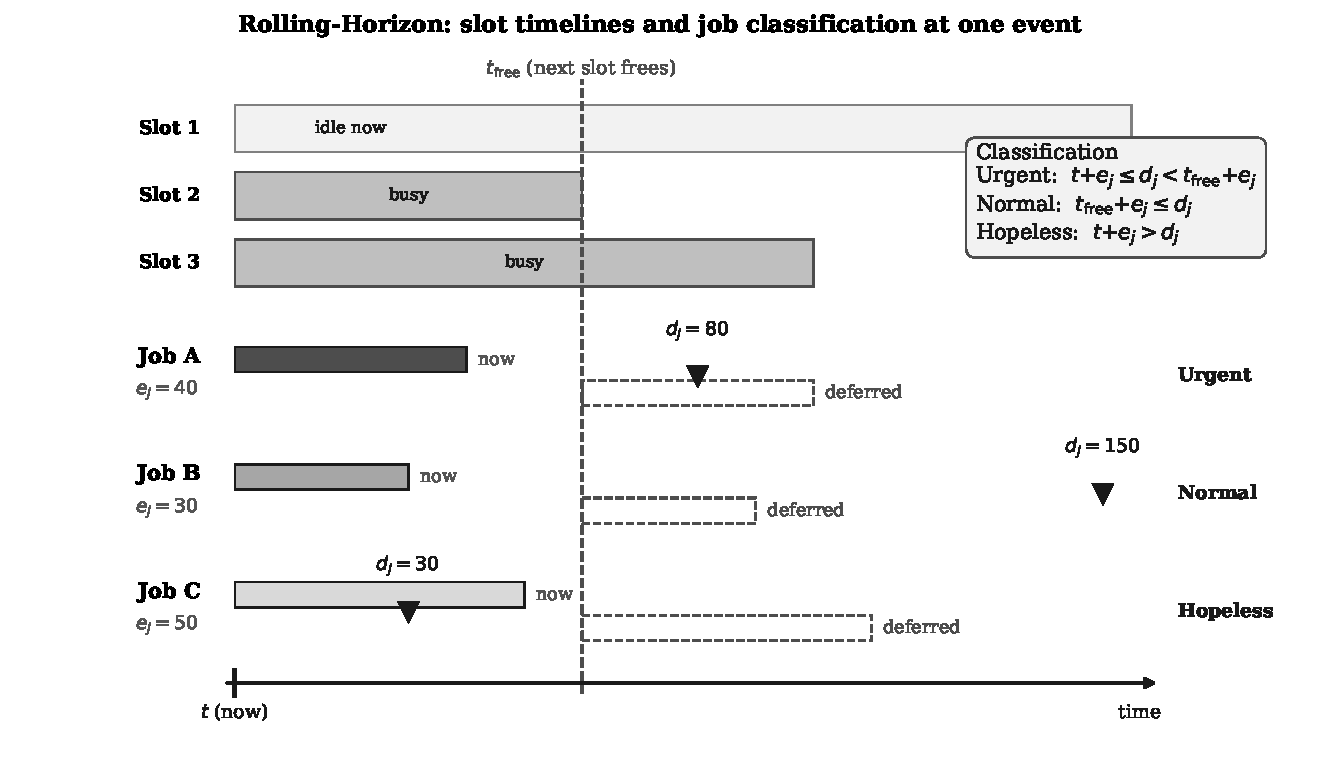
\includegraphics[width=0.98\linewidth,height=0.90\textheight,keepaspectratio]{figures/rh_timeline.pdf}
\caption[Rolling-Horizon slot timelines and job classification]{Rolling-Horizon slot timelines and job classification.}
\label{fig:rh-timeline}
\end{figure}
\end{landscape}

The RH scheduler is implemented in \texttt{CGRSP/\allowbreak cgrsp/\allowbreak schedulers/\allowbreak rolling\allowbreak\_horizon\allowbreak\_scheduler.py}. Anticipation is enabled ($\rho_{\text{res}}=1$, load-gated) in all experiments; because the gate disables it under saturation, the baseline hectic-day results ($C_{\max}=5$) are identical to the plain forward-simulation policy (at $C_{\max}\ge 8$ the offered load falls below the gate and anticipation is active), while the surge day exhibits its benefit and the monthly results, whose calendar is mostly below the gate, carry it throughout. The reservation count and the gate are examined in Section~\ref{ssec:anticipation-reservation-sensitivity}.

\subsection{CADR: Cost-Aware Deadline-Risk}
\label{ssec:cadr-cost-aware-deadline-risk}

The Cost-Aware Deadline-Risk (CADR) scheduler is the second scheduling contribution of this work. Like RH, CADR classifies waiting jobs into tiers based on deadline urgency; unlike RH, it uses a scale-free critical ratio rather than a forward-simulation timeline, and it integrates cost-aware node selection as a secondary objective.

\textbf{Critical ratio.} The critical ratio is a classical dispatching rule from the operations-research literature~\cite{pinedo2016scheduling}; the contribution here is its combination with the scale-free three-tier triage, doomed-last demotion, and stock-filtered cheapest-deadline-feasible placement. For each job $j$ at scheduling time $t$ with estimated service time $e_j = \min_{m \in I} \overline{W}(\kappa_j, g(m))$, the critical ratio is:
\begin{equation}
\mathrm{CR}_j(t) = \frac{d_j - t}{e_j}
\label{eq:cr}
\end{equation}
A ratio $\mathrm{CR}_j \leq 1$ means the remaining time is at most the estimated service time, so immediate dispatch leaves no estimated slack for provisioning; a shorter realised service time may still meet the deadline. Such jobs enter the last tier. $\mathrm{CR}_j = \mathrm{CR}^*$ is the boundary between at-risk and safe jobs, with a baseline $\mathrm{CR}^* = 3$.

\textbf{Three-tier classification.} At each scheduling event the waiting queue is partitioned by the critical ratio (Eq.~\ref{eq:cr}) into three tiers (Figure~\ref{fig:cadr-triage}a):
\begin{itemize}
  \item \textbf{Doomed under the estimate} ($\mathrm{CR}_j \leq 1$): immediate dispatch is projected to miss; dispatched \emph{last} to prioritise jobs projected to meet their deadlines.
  \item \textbf{At-risk} ($1 < \mathrm{CR}_j \leq \mathrm{CR}^*$): deadline is reachable but slack is tight; dispatched in earliest-deadline-first (EDF) order.
  \item \textbf{Safe} ($\mathrm{CR}_j > \mathrm{CR}^*$): ample slack remaining; dispatched in shortest-processing-time (SPT) order to minimise mean wait.
\end{itemize}

\textbf{Cost-aware node selection.} Within a placement (Figure~\ref{fig:cadr-triage}b), CADR first restricts the capable nodes to those not currently low on stock (falling back to all capable nodes only when every capable node is low-stock, since low stock signals a longer expected provisioning delay), then selects the cheapest among them whose estimated finish time satisfies the deadline (deadline-feasible cheapest node). If no deadline-feasible node exists, it falls back to the fastest node in the same stock-filtered pool. This integrates cost awareness directly into dispatch rather than as a post-hoc re-scoring.



\textbf{Why CADR has lower tardiness than RH.} Both schedulers demote on an instantaneous test (RH: $t + e_j > d_j$; CADR: $\mathrm{CR}_j \leq 1$), and both dispatch demoted jobs last in deadline order. Because both take $e_j$ over the idle slots and RH's strict test $t + e_j > d_j$ implies $\mathrm{CR}_j \leq 1$, any job RH demotes at a given instant CADR demotes too, so the difference does not lie in demotion. It lies in promotion. Under saturation RH moves a job into its urgent tier only when it can no longer wait for the next slot to free ($t_{\text{free}} + e_j > d_j$), a window of roughly one service time that is planned without the provisioning delay. A tight job not dispatched inside that window becomes hopeless and waits behind the loose backlog, so RH's missed jobs are frequently tight jobs that finish hours late. CADR's at-risk tier opens at $\mathrm{CR}_j \leq \mathrm{CR}^* = 3$, about three service times before the deadline, so tight jobs are dispatched with margin, and its missed jobs are almost all loose jobs that finish modestly late. As a result, CADR gives substantially lower mean tardiness than RH while keeping the miss count nearly as low.

\textbf{Ablation variant.} The CADR-order-only (CADR-OO) variant retains the three-tier critical-ratio ordering but replaces cost-aware node selection with fastest-available-node placement within the stock-filtered pool. This isolates the contribution of the cost-aware placement component from the ordering component (Section~\ref{sec:ablation-analysis}).

\begin{algorithm}[H]
\caption{CADR Scheduler}
\label{alg:cadr}
\begin{algorithmic}[1]
\REQUIRE Queue $Q$; idle node set $I$; current time $t$; threshold $\mathrm{CR}^*=3$
\FOR{each job $j \in Q$}
  \STATE $e_j \leftarrow \min_{m \in I} \overline{W}(\kappa_j, g(m))$
  \STATE $\mathrm{CR}_j \leftarrow (d_j - t) / e_j$
\ENDFOR
\STATE $Q_{\text{doomed}} \leftarrow \{j \in Q : \mathrm{CR}_j \leq 1\}$, ordered last
\STATE $Q_{\text{atrisk}} \leftarrow \{j \in Q : 1 < \mathrm{CR}_j \leq \mathrm{CR}^*\}$, sorted by $d_j$ ascending (EDF)
\STATE $Q_{\text{safe}}   \leftarrow \{j \in Q : \mathrm{CR}_j > \mathrm{CR}^*\}$, sorted by $e_j$ ascending (SPT)
\FOR{each job $j$ in $Q_{\text{atrisk}} \mathbin{\|} Q_{\text{safe}} \mathbin{\|} Q_{\text{doomed}}$}
  \IF{$I = \emptyset$} \STATE \textbf{break} \ENDIF
  \STATE $I' \leftarrow \{m \in I : s_{g(m)}(t) \neq \text{Low}\}$; \quad \textbf{if} $I' = \emptyset$ \textbf{then} $I' \leftarrow I$ \COMMENT{stock-filtered pool}
  \STATE $I_{\text{feasible}} \leftarrow \{m \in I' : t + \overline{W}(\kappa_j, g(m)) \leq d_j\}$ \COMMENT{deadline-feasible nodes}
  \IF{$I_{\text{feasible}} \neq \emptyset$}
    \STATE $m^* \leftarrow \arg\min_{m \in I_{\text{feasible}}} p_{g(m)}$ \COMMENT{cheapest per-second rate, ties by exec time}
  \ELSE
    \STATE $m^* \leftarrow \arg\min_{m \in I'} \overline{W}(\kappa_j, g(m))$ \COMMENT{fastest fallback in the stock-filtered pool}
  \ENDIF
  \STATE Assign $j \to m^*$; remove $m^*$ from $I$
\ENDFOR
\end{algorithmic}
\end{algorithm}

\begin{landscape}
\begin{figure}[H]
\centering
\captionsetup{font=small,skip=6pt}
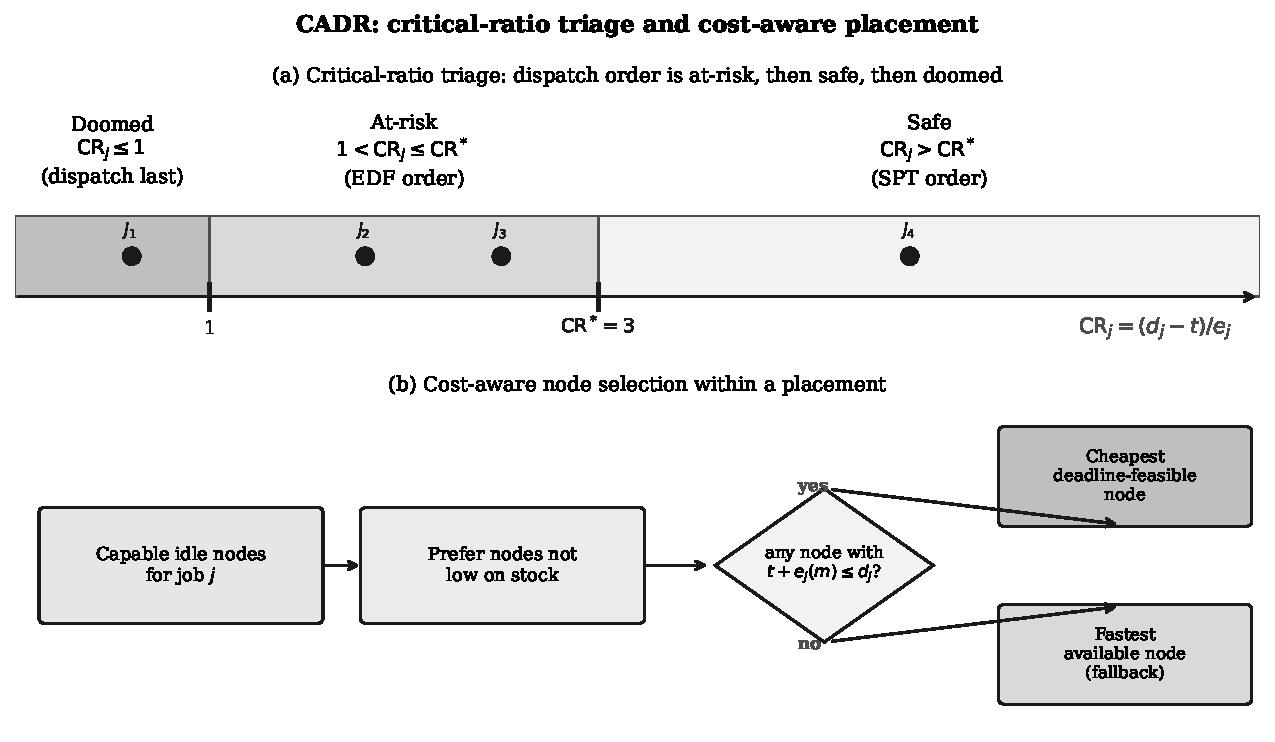
\includegraphics[width=0.98\linewidth,height=0.72\textheight,keepaspectratio]{figures/cadr_triage.pdf}
\caption[CADR critical-ratio triage and cost-aware placement]{CADR scheduling mechanics. Panel~(a): the critical ratio $\mathrm{CR}_j = (d_j - t)/e_j$ places every queued job on a scale-free axis partitioned into three tiers: doomed ($\mathrm{CR}_j \leq 1$, dispatched last), at-risk ($1 < \mathrm{CR}_j \leq \mathrm{CR}^*$, EDF order), and safe ($\mathrm{CR}_j > \mathrm{CR}^*$, SPT order); example jobs $j_1$ to $j_4$ illustrate the triage. Panel~(b): within each placement, node selection prefers non-low-stock nodes and picks the cheapest deadline-feasible node, falling back to the fastest available node when no node can meet the deadline.}
\label{fig:cadr-triage}
\end{figure}
\end{landscape}

Algorithm~\ref{alg:cadr} summarises the full procedure; the implementation is in \texttt{CGRSP/\allowbreak cgrsp/\allowbreak schedulers/\allowbreak cost\allowbreak\_aware\allowbreak\_deadline\allowbreak\_risk.py}. The critical-ratio threshold $\mathrm{CR}^*=3$ is the baseline; its sensitivity is examined in Section~\ref{ssec:critical-ratio-threshold-sensitivity}.

\subsection{Adaptive: Queue-Pressure EDF-SPT Hybrid}
\label{ssec:adaptive-queue-pressure-edf-spt-hybrid}

The Adaptive scheduler is a third hybrid policy, evaluated alongside RH and CADR to test the alternative ``adaptive SPT-EDF hybrid'' design. Like SPT+Rescue it uses a laxity threshold to separate urgent from non-urgent jobs, but it adds two refinements: a \emph{hopeless} tier that demotes jobs projected to miss under the service-time estimate (as in RH and CADR), and a \emph{queue-pressure} rule that widens the urgent tier as the backlog grows, so the policy interpolates between SPT under light load and EDF under heavy load.

At each scheduling event the laxity of job $j$ is computed exactly as in SPT+Rescue (Eq.~\ref{eq:laxity}), $L_j(t) = d_j - t - \min_{m \in I} \overline{W}(\kappa_j, g(m))$, and the queue is partitioned into three tiers against an \emph{effective} threshold $\theta_{\text{eff}}$:
\begin{itemize}
  \item \textbf{Critical} ($0 \leq L_j < \theta_{\text{eff}}$): dispatched first, in earliest-deadline (EDF) order.
  \item \textbf{Safe} ($L_j \geq \theta_{\text{eff}}$): dispatched next, in shortest-processing-time (SPT) order.
  \item \textbf{Hopeless under the estimate} ($L_j < 0$): projected to miss even if dispatched now; dispatched last (EDF order within the tier) to prioritise work projected to meet its deadline.
\end{itemize}
The queue-pressure adaptation sets $\theta_{\text{eff}} = \theta$ (baseline $600$\,s) under normal load, but expands it to the full loose-deadline window ($\theta_{\text{eff}} = T_{\text{loose}} = 28{,}800$\,s, a fixed constant in the implementation) whenever the waiting queue exceeds a pressure threshold $P$ (baseline $10$ jobs). Under that expansion every job with positive laxity falls into the critical tier, so the policy reduces to EDF ordering with hopeless-demotion exactly when the system is congested, the regime in which deadline ordering is most valuable; when the backlog is short it behaves as SPT for the safe majority. Critical-tier jobs are placed on the fastest deadline-reliable node (with a stock and provisioning-reliability penalty), while safe-tier jobs use the same speed-weighted cost-aware node score as SPT (Eq.~\ref{eq:spt_score}).

\begin{algorithm}[H]
\caption{Adaptive EDF-SPT Hybrid Scheduler}
\label{alg:adaptive}
\begin{algorithmic}[1]
\REQUIRE Queue $Q$; idle node set $I$; current time $t$; threshold $\theta$; pressure $P$
\STATE $\theta_{\text{eff}} \leftarrow T_{\text{loose}}$ \textbf{if} $|Q| > P$ \textbf{else} $\theta$ \COMMENT{queue-pressure widening}
\FOR{each job $j \in Q$}
  \STATE $e_j \leftarrow \min_{m \in I} \overline{W}(\kappa_j, g(m))$; \quad $L_j \leftarrow d_j - t - e_j$
\ENDFOR
\STATE $Q_{\text{crit}} \leftarrow \{j : 0 \leq L_j < \theta_{\text{eff}}\}$ sorted by $d_j$ (EDF)
\STATE $Q_{\text{safe}} \leftarrow \{j : L_j \geq \theta_{\text{eff}}\}$ sorted by $e_j$ (SPT)
\STATE $Q_{\text{hope}} \leftarrow \{j : L_j < 0\}$ sorted by $d_j$, ordered last
\FOR{each job $j$ in $Q_{\text{crit}} \mathbin{\|} Q_{\text{safe}} \mathbin{\|} Q_{\text{hope}}$}
  \IF{$I = \emptyset$} \STATE \textbf{break} \ENDIF
  \STATE $m^* \leftarrow$ fastest reliable node if $j$ critical (exec time plus stock penalty $\{0, 50, 200\}$\,s and per-type reliability prior $\{$A4000 0, A4500 5, A5000 15, 3090 40$\}$\,s), else speed-weighted cost-aware node (Eq.~\ref{eq:spt_score})
  \STATE Assign $j \to m^*$; remove $m^*$ from $I$
\ENDFOR
\end{algorithmic}
\end{algorithm}

Algorithm~\ref{alg:adaptive} summarises the procedure; the implementation is in \texttt{CGRSP/\allowbreak cgrsp/\allowbreak schedulers/\allowbreak adaptive\allowbreak\_scheduler.py}. It differs from RH in that its tier boundary is driven by an instantaneous laxity-and-queue-length rule rather than a forward-simulation timeline, and from CADR in that it uses an absolute laxity threshold rather than a scale-free critical ratio. Its empirical behaviour relative to RH and CADR is reported in Chapter~\ref{chap:experiments}.

\subsection{Ten-Policy Decision Snapshot}
\label{ssec:ten-policy-decision-snapshot}

Figure~\ref{fig:snapshot-decision} makes the decision-level difference concrete. It freezes one queue and fleet state at $t=600$\,s and presents it unchanged to all ten schedulers. Nine jobs wait; three slots are idle (A4000 and A4500 at High stock, A5000 at Medium) and two are busy (RTX~3090 and A4000). Under the mean service-time estimate on the fastest idle node, J1 and J8 can still meet their deadlines, J2 and J7 cannot even if dispatched immediately, and J3 to J6 and J9 have loose deadlines. The snapshot is illustrative, not a simulation result: it uses the same execution-time model and scheduler code as the experiments, but it is a single hand-chosen state.

FIFO, LCF and Balanced fill the three slots with loose jobs (J3 to J5), ignoring deadline risk. SPT serves J8 but spends the other two slots on loose jobs J3 and J6. EDF and SPT+Rescue dispatch J7 and J2, both already infeasible under the estimate, before J8: their urgent tier sorts by deadline, so the two earliest deadlines consume two slots even though neither job can be saved under the estimate. Random sends J7, J8 and J4. Adaptive, RH and CADR all leave J2 and J7 queued, dispatch both feasible tight jobs J1 and J8, and give the third slot to a loose job.

The difference is not node choice: all three idle slots are deadline-feasible for the feasible tight jobs, and the three policies that serve both differ only in which type receives which job. The gain comes from the ordering: not spending capacity on jobs that cannot meet their deadlines, and promoting the two feasible tight jobs. This is the mechanism behind the aggregate miss differences in Chapter~\ref{chap:experiments}; the snapshot shows why deadline-aware demotion matters, not that any one policy wins on every event.

\begin{figure}[H]
\centering
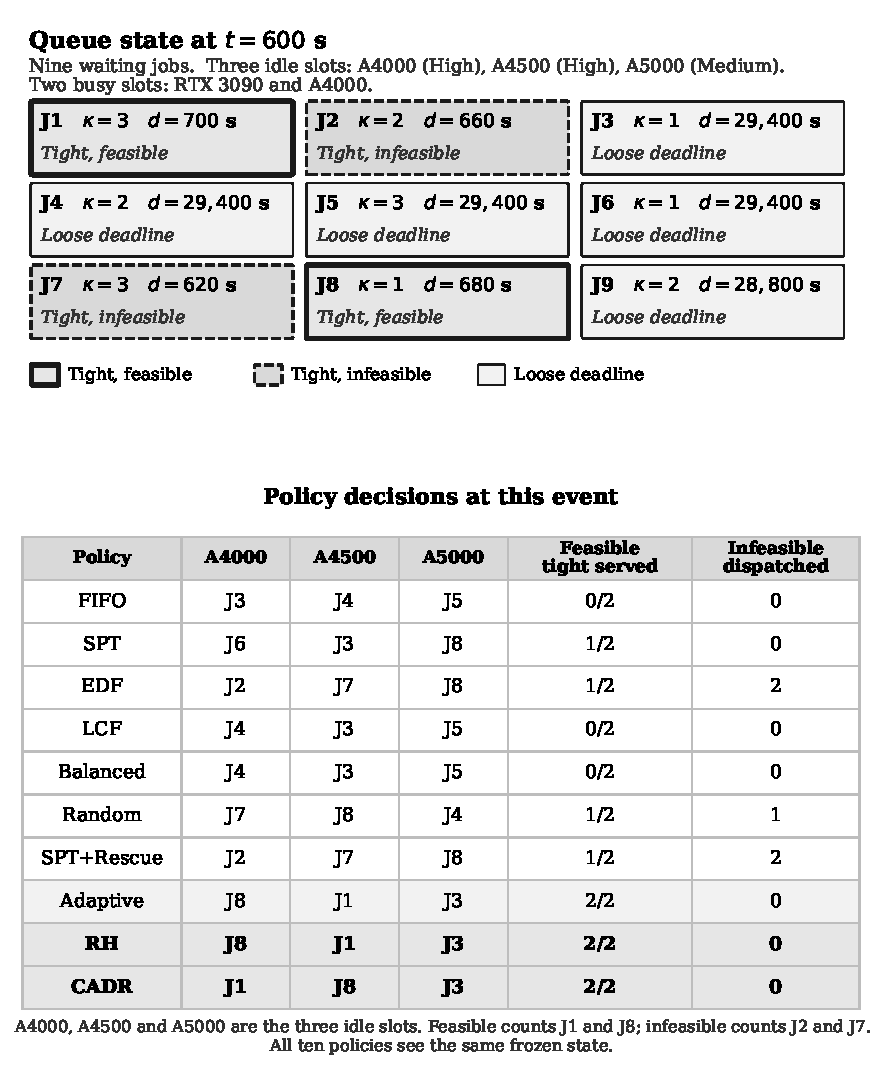
\includegraphics[width=\linewidth]{figures/snapshot_decision.pdf}
\caption[Frozen ten-policy decision snapshot]{Frozen ten-policy decision snapshot. The same queue and fleet state is presented to all ten schedulers at $t=600$\,s: nine waiting jobs, three idle slots (A4000, A4500, A5000) and two busy slots. Border weight and line style mark the tight jobs that can still meet their deadlines (J1, J8) and those that cannot under mean service times (J2, J7); the remaining jobs have loose deadlines. The table reports the job each policy assigns to each idle slot. This is an illustrative snapshot using the simulator's execution-time model and scheduler implementations, not a simulation run or a statistical result.}
\label{fig:snapshot-decision}
\end{figure}

\section{Metrics Collection}
\label{sec:metrics-collection}

The simulator records per-job metrics at the time of job completion:
\begin{itemize}
  \item $t_j^{\text{submit}}$, $t_j^{\text{start}}$, $t_j^{\text{complete}}$: timestamps in seconds
  \item $w_j = t_j^{\text{start}} - t_j^{\text{submit}}$: waiting time (Eq.~\ref{eq:wait})
  \item $r_j = t_j^{\text{complete}} - t_j^{\text{submit}}$: response time (Eq.~\ref{eq:resp}), tracked as a diagnostic; Chapter~\ref{chap:experiments} reports it through its two components rather than as a separate table column, since $r_j$ differs from the tabulated waiting time $w_j$ only by the realised execution time, whose per-policy differences enter through the cost metric
  \item $\delta_j = \mathbf{1}[t_j^{\text{complete}} \leq d_j]$: deadline adherence indicator (Eq.~\ref{eq:adherence}); the miss indicator is $1 - \delta_j$, and the miss rate is $\Delta_{\text{miss}} = \frac{1}{|\calJ|}\sum_{j}(1-\delta_j)$ (Eq.~\ref{eq:missrate})
  \item $c_j = W(\kappa_j, g_j) \cdot p_{g_j}$: job execution cost (Eq.~\ref{eq:cost_cost})
\end{itemize}

Fleet utilisation is recorded as an event-sampled series (one sample per processed event) together with a time series of idle and running slot counts; per-job provisioning delay is recoverable from each dispatch record as the gap between dispatch and execution start. All metrics are reported at the end of the simulation via \texttt{get\_\allowbreak metrics\_\allowbreak summary()}, which returns a structured dictionary used both for JSON export and for the PDF report generator.

Part of the verification half of the V\&V framework adopted in Chapter~\ref{chap:related} is executed rather than merely asserted. A constraint verifier re-checks completed runs on the seed-42 hectic-day workload against three model constraints: the seven baseline policies in the Phase~2 benchmark itself, and RH, CADR and the Adaptive hybrid in a companion run on the identical workload (\texttt{verify\_proposed.py}). Two of the checks are recomputed from the recorded per-job data rather than read from the accumulators that produced the summary: that every job's deadline-adherence flag agrees with its own recorded completion time and deadline, and that the reported miss count agrees with those flags; and that each job's cost equals $W(\kappa_j, g_j) \cdot p_{g_j}$. The third, that each job is dispatched once and each node holds at most one job at a time, is checked against a dispatch log that records every dispatch and is never overwritten. A job dispatched other than exactly once is a violation, as is any mismatch between the completion counter and the number of completed jobs, and no slot may hold two jobs whose occupancy intervals $[t_j^{\text{dispatch}}, t_j^{\text{complete}})$ overlap, provisioning wait included, which is Constraint~(\ref{eq:single_job_node}) itself; a job still held at the end of a run occupies its slot from dispatch onwards. All three checks report zero violations, over all 950 jobs, for all ten schedulers (in the \texttt{verification} block of the Phase~2 \texttt{report.json} and in \texttt{verification\_proposed.json}).
